\documentclass[aspectratio=169]{beamer}

\usetheme{Madrid}

\usepackage{graphicx}
\usepackage{tikz}
\usetikzlibrary{decorations.pathreplacing,positioning}
\usepackage{booktabs}
\usepackage[round,authoryear]{natbib}

\setbeamertemplate{navigation symbols}{}
\newenvironment{bluealertblock}[1]{%
    \begingroup
    \setbeamercolor{block title alerted}{use=structure,fg=white,bg=structure.fg}%
    \setbeamercolor{block body alerted}{use=structure,fg=black,bg=structure.fg!10!white}%
    \begin{alertblock}{#1}
}{%
    \end{alertblock}
    \endgroup
}

\title{Chevalier and Scharfstein (1996)}
\author{Siddhartha Lewis-Hayre}
\date{\today}

\begin{document}

\begin{frame}
    \titlepage
\end{frame}

\begin{frame}{Motivation}
    \begin{itemize}
        \item Countercyclicality of markups are central in New Keynesian DSGE models
        \begin{itemize}
            \item Adding aggregate demand shocks to RBC model makes wages countercyclical, contrary to empirical evidence
            \item Countercyclical markups could nullify this effect
        \end{itemize}
    \end{itemize}

    \vspace{0.1cm}

    \begin{columns}[c,onlytextwidth]
        \begin{column}{0.49\textwidth}
            \centering
            \textbf{Positive shock to aggregate demand}

            \resizebox{0.88\linewidth}{!}{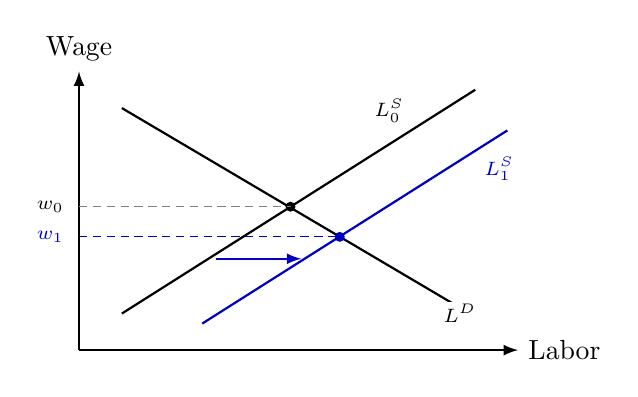
\begin{tikzpicture}[x=0.68cm,y=0.58cm,>=latex]
    \draw[->,thick] (0,0) -- (8.2,0) node[right] {Labor};
    \draw[->,thick] (0,0) -- (0,6.1) node[above] {Wage};

    % Initial labor supply and the fixed MPL schedule (labor demand).
    \draw[thick] (0.8,0.8) -- (7.4,5.7)
        node[pos=0.82,above left=2pt,font=\scriptsize,fill=white,inner sep=1pt] {$L^S_0$};
    \draw[thick] (0.8,5.3) -- (7.3,0.8)
        node[pos=0.88,below right=6pt,font=\scriptsize,fill=white,inner sep=1pt] {$L^D$};

    % The aggregate-demand change shifts labor supply to the right.
    \draw[blue!75!black,thick] (2.3,0.58) -- (8.0,4.81)
        node[pos=0.90,below right=2pt,font=\scriptsize,fill=white,inner sep=1pt] {$L^S_1$};

    \coordinate (EzeroAD) at (3.95,3.14);
    \coordinate (Ead) at (4.87,2.48);
    \fill (EzeroAD) circle (1.8pt);
    \fill[blue!75!black] (Ead) circle (1.8pt);

    \draw[densely dashed,gray] (0,3.14) -- (EzeroAD)
        node[pos=0,left=2pt,font=\scriptsize,text=black] {$w_0$};
    \draw[densely dashed,blue!75!black] (0,2.48) -- (Ead)
        node[pos=0,left=2pt,font=\scriptsize,text=blue!75!black] {$w_1$};
    \draw[->,blue!75!black,thick] (2.55,2.0) -- (4.15,2.0);
\end{tikzpicture}
}
        \end{column}
        \begin{column}{0.49\textwidth}
            \centering
            \textbf{Negative shock to markup}

            \resizebox{0.88\linewidth}{!}{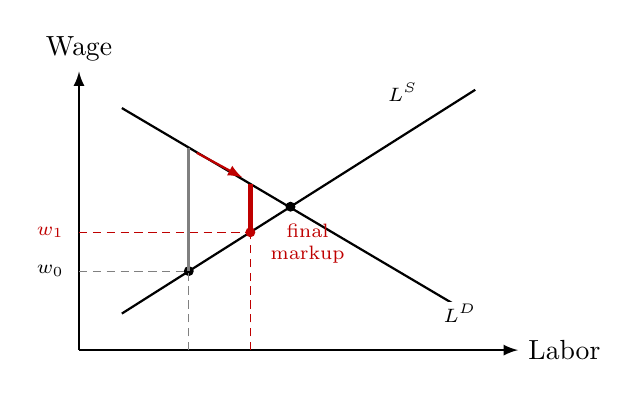
\begin{tikzpicture}[x=0.68cm,y=0.58cm,>=latex]
    \draw[->,thick] (0,0) -- (8.2,0) node[right] {Labor};
    \draw[->,thick] (0,0) -- (0,6.1) node[above] {Wage};

    % Labor supply and labor demand
    \draw[thick] (0.8,0.8) -- (7.4,5.7)
        node[pos=0.88,above left=6pt,font=\scriptsize,fill=white,inner sep=1pt] {$L^S$};
    \draw[thick] (0.8,5.3) -- (7.3,0.8)
        node[pos=0.88,below right=6pt,font=\scriptsize,fill=white,inner sep=1pt] {$L^D$};

    % Competitive equilibrium
    \coordinate (Ecompetitive) at (3.95,3.14);
    \fill (Ecompetitive) circle (1.8pt);

    % Initial high-markup quantity and wage (the wage lies on labor supply).
    \coordinate (LinitialDemand) at (2.05,4.43);
    \coordinate (LinitialSupply) at (2.05,1.73);
    \fill (LinitialSupply) circle (1.8pt);
    \draw[densely dashed,gray] (0,1.73) -- (LinitialSupply)
        node[pos=0,left=2pt,font=\scriptsize,text=black] {$w_0$};
    \draw[densely dashed,gray] (2.05,0) -- (LinitialDemand);

    % Lower markup: employment moves right and the wage rises along labor supply.
    \coordinate (LfinalDemand) at (3.20,3.64);
    \coordinate (LfinalSupply) at (3.20,2.58);
    \fill[red!75!black] (LfinalSupply) circle (1.8pt);
    \draw[densely dashed,red!75!black] (0,2.58) -- (LfinalSupply)
        node[pos=0,left=2pt,font=\scriptsize,text=red!75!black] {$w_1$};
    \draw[densely dashed,red!75!black] (3.20,0) -- (LfinalDemand);
    \draw[->,red!75!black,thick] (2.20,4.32) -- (3.05,3.78);

    % The markup is the wedge between labor demand and labor supply.
    \draw[gray,line width=1.2pt] (LinitialSupply) -- (LinitialDemand);
    \draw[red!75!black,line width=2pt] (LfinalSupply) -- (LfinalDemand)
        node[midway,right=3pt,yshift=-13pt,font=\scriptsize,align=center,text=red!75!black]
        {final\\markup};
\end{tikzpicture}
}
        \end{column}
    \end{columns}

    \begin{alertblock}{Question}
        Why might markups be countercyclical?
    \end{alertblock}
\end{frame}

\begin{frame}{Contribution}
    \begin{itemize}
        \item Three reasons why markups might be countercyclical
        \begin{enumerate}
            \item elasticity of demand changes with output
            \item collusion is more difficult during booms 
            \begin{itemize}
                \item Rotemberg and Woodford (1991, 1992)
            \end{itemize}
            \item \textbf{capital market imperfections}
        \end{enumerate}
    \end{itemize}

    \vspace{0.15cm}

    \begin{bluealertblock}{Contribution}
        Explains countercyclicality of markups with financial frictions
    \end{bluealertblock}

    \vspace{0.3cm}

    Provides empirical evidence from supermarket industry
\end{frame}

\begin{frame}{Literature}
    Relation to the macro-literature:
    \vspace{0.3cm}
    \begin{itemize}
        \item Capital market imperfections reverses Rotemberg and Woodford (1991, 1992) result that collusion is more difficult during booms
        \item Sticky wages and Calvo pricing were later introduced to yield countercyclical markups
        \begin{itemize}
            \item See for example: Yun (1996) and Rotemberg and Woodford (1997)
        \end{itemize}
        \item Like Bernanke, Gertler and Gilchrist (1998), uses financial friction to get amplification
        \item Gilchrist, Schoenle, Sim and Zakraj\v{s}ek (2017) argue financial frictions can strengthen countercyclical markups
    \end{itemize}
    
\end{frame}

\begin{frame}{Results}
\textbf{Theoretical:}
\begin{itemize}
    \item Findings:
    \begin{itemize}
        \item firm's markup more counter-cyclical if financially constrained
        \item firm's markup more counter-cyclical if rival is financially constrained
        \item industry-wide markups more counteryclical if more firms are financially constrained
    \end{itemize}
    \item Mechanism:
    \begin{itemize}
        \item if a firm needs external financing, then a bust will cause the firm to be siezed
        \item so future profits will not matter as much and firm will increase price today
    \end{itemize} 
\end{itemize}

\vspace{0.3cm}

\textbf{Empirical:}
\begin{itemize}
    \item after oil shock, prices fall less where local and regional chains have larger prescense
    \item chains that undertook LBOs cut prices less during 1990-1991 macroeconomic recession
    \item in poorly performing cities following 1990-1991 macro-recession
    \begin{itemize}
        \item leveraged firms cut prices by less
        \item firms cut prices less if their rivals were highly leveraged
    \end{itemize}
\end{itemize}

\end{frame}


\begin{frame}{Model}
    \begin{columns}[T,onlytextwidth]
        \begin{column}{0.49\textwidth}
            \begin{itemize}
                \item Two-period model
                \item In first period, firms compete for customers by setting prices
                \begin{itemize}
                    \item Discrete choice where agents get value from being ``closer" to a firm
                \end{itemize}
                \item In second period, firms keep customers from first period
                \begin{itemize}
                    \item motiviated by switching costs
                \end{itemize}
            \end{itemize}
        \end{column}
        \begin{column}{0.49\textwidth}
            \raggedleft
            \resizebox{!}{0.43\textheight}{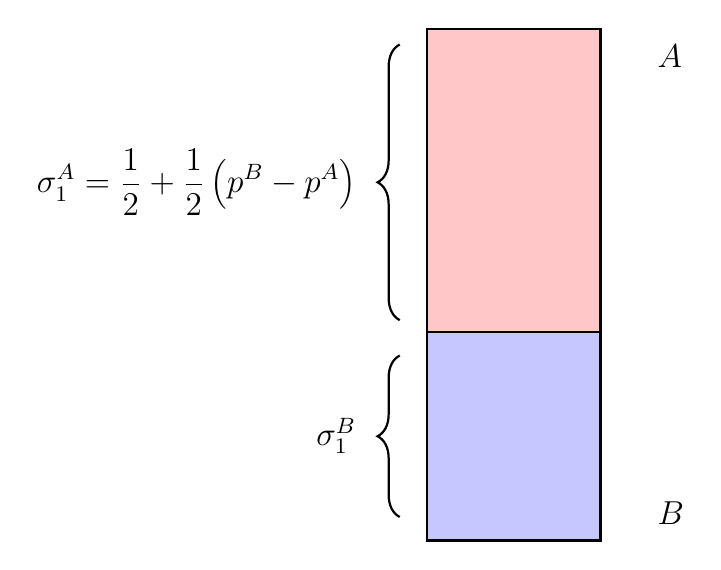
\begin{tikzpicture}[
    every node/.style={font=\large}
]

% Main rectangle
\fill[red!22] (0,2.65) rectangle (2.2,6.5);
\fill[blue!22] (0,0) rectangle (2.2,2.65);
\draw[thick] (0,0) rectangle (2.2,6.5);

% Divider between A and B
\draw[thick] (0,2.65) -- (2.2,2.65);

% Labels A and B
\node[right] at (2.8,6.15) {$A$};
\node[right] at (2.8,0.35) {$B$};

% Braces on left
\draw[
    decorate,
    decoration={brace, amplitude=8pt},
    thick
]
(-0.35,2.8) -- (-0.35,6.3)
node[midway,left=12pt]
{$\displaystyle \sigma_1^A=\frac{1}{2}
  +\frac{1}{2}\left(p^B-p^A\right)$};

\draw[
    decorate,
    decoration={brace, amplitude=8pt},
    thick
]
(-0.35,0.3) -- (-0.35,2.35)
node[midway,left=12pt] {$\sigma_1^B$};

\end{tikzpicture}
}
        \end{column}
    \end{columns}

    \vspace{0.35cm}
    \centering
    \resizebox{0.88\linewidth}{!}{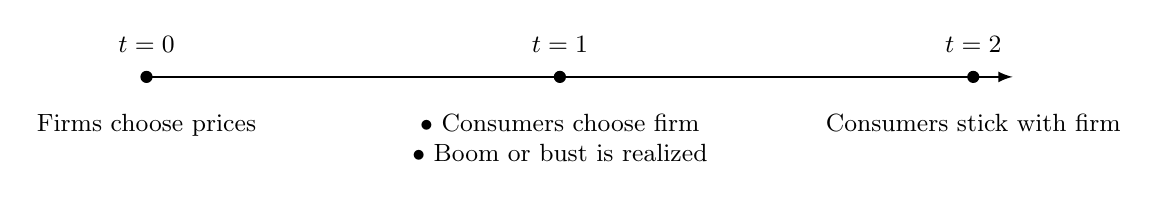
\begin{tikzpicture}[
    >=latex,
    every node/.style={font=\small},
    event/.style={align=center}
]
    % Timeline
    \draw[->,thick] (0,0) -- (11,0);

    % Period markers
    \foreach \x/\t in {0/0,5.25/1,10.5/2} {
        \fill (\x,0) circle (2.2pt);
        \node[above=0.18cm] at (\x,0) {$t=\t$};
    }

    % Events
    \node[event,below=0.35cm] at (0,0)
        {Firms choose prices};
    \node[event,below=0.35cm] at (5.25,0)
        {$\bullet$ Consumers choose firm\\$\bullet$ Boom or bust is realized};
    \node[event,below=0.35cm] at (10.5,0)
        {Consumers stick with firm};
\end{tikzpicture}
}
\end{frame}

\begin{frame}{Financial Friction}
    What if firm needs external financing?
    \begin{itemize}
        \item Cash flow from firm is observable but not ``verifiable''
        \item Moral hazard problem where manager can divert cash flow to herself
        \item Investor can force liquidation value and recover $\lambda$ of cash flows
    \end{itemize}
    
    \vspace{0.1cm}

    Hart and Moore (1989), Bolton and Scharfstein (1990, 1996) show optimal contract is debt where investor siezes firm if it does not pay

    \vspace{0.1cm}

    Assumptions:
    \begin{itemize}
        \item The contract is incentive compatible
        \begin{itemize}
            \item $D \leq \pi^k_2(\sigma_1^k)$
        \end{itemize}
        \item The manager repays in a boom and defaults in a bust
        \begin{itemize}
            \item $\pi^k_1(\theta_H) > D > \pi^k_1(\theta_L)$
        \end{itemize}
    \end{itemize}
    \vspace{0.1cm}

    \begin{bluealertblock}{Takeaway}
        Firm does not get second period payoff if bad state arrives
    \end{bluealertblock}
\end{frame}

\begin{frame}{Financial Constraint}
    \begin{columns}[T,onlytextwidth]
        \begin{column}{0.49\textwidth}
            \centering
            \textbf{Unconstrained firm}

            \vspace{0.25cm}
            \resizebox{\linewidth}{!}{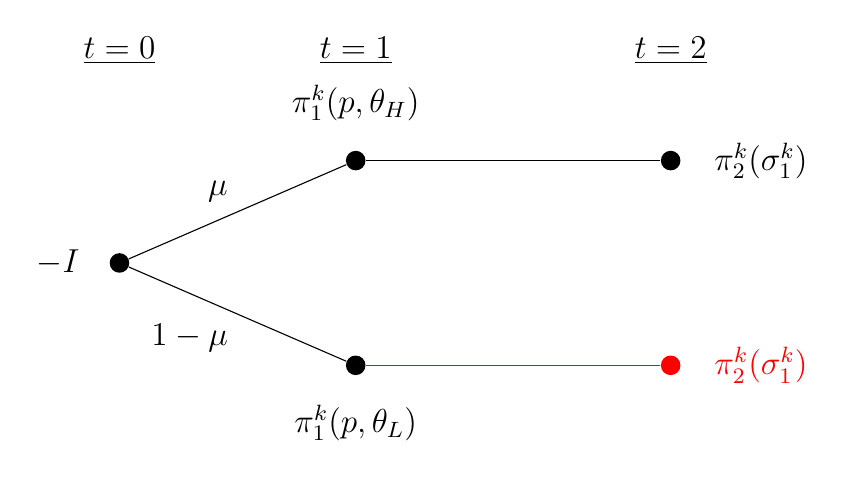
\begin{tikzpicture}[
    >=stealth,
    every node/.style={font=\large},
    dot/.style={circle, fill=black, inner sep=2.5pt}
]

% Time labels
\node at (1,5.2) {$\underline{t=0}$};
\node at (4,5.2) {$\underline{t=1}$};
\node at (8,5.2) {$\underline{t=2}$};

% Nodes
\node[dot] (start) at (1,2.5) {};
\node[dot] (up1)   at (4,3.8) {};
\node[dot] (down1) at (4,1.2) {};
\node[dot] (up2)   at (8,3.8) {};
\node[dot, fill=red] (down2) at (8,1.2) {};

% Initial investment
\node[left=0.25cm of start] {$-I$};

% Branches from initial choice
\draw (start) -- (up1)
    node[midway, above left] {$\mu$};

\draw (start) -- (down1)
    node[midway, below left] {$1-\mu$};

% Period 1 payoffs
\node[above=0.25cm of up1]
    {$\pi_1^k(p,\theta_H)$};

\node[below=0.25cm of down1]
    {$\pi_1^k(p,\theta_L)$};

% Period 1 -> Period 2
\draw (up1) -- (up2);
\draw[red] (down1) -- (down2);

% Period 2 payoffs
\node[right=0.3cm of up2]
    {$\pi_2^k(\sigma_1^k)$};

\node[right=0.3cm of down2, text=red]
    {$\pi_2^k(\sigma_1^k)$};

\end{tikzpicture}
}
        \end{column}
        \begin{column}{0.49\textwidth}
            \centering
            \textbf{Financially constrained firm}

            \vspace{0.25cm}
            \resizebox{0.90\linewidth}{!}{\begin{tikzpicture}[
    >=stealth,
    every node/.style={font=\large},
    dot/.style={circle, fill=black, inner sep=2.5pt}
]

% Time labels
\node at (1,5.2) {$\underline{t=0}$};
\node at (4,5.2) {$\underline{t=1}$};
\node at (8,5.2) {$\underline{t=2}$};

% Nodes
\node[dot] (start) at (1,2.5) {};
\node[dot] (up1)   at (4,3.8) {};
\node[dot] (down1) at (4,1.2) {};
\node[dot] (up2)   at (8,3.8) {};

% Branches from initial choice
\draw (start) -- (up1)
    node[midway, above left] {$\mu$};

\draw (start) -- (down1)
    node[midway, below left] {$1-\mu$};

% Period 1 payoffs
\node[above=0.25cm of up1]
    {$\pi_1^k(p,\theta_H)-D$};

\node[below=0.25cm of down1]
    {$\pi_1^k(p,\theta_L)$};

% Only the high-state branch continues to period 2.
\draw (up1) -- (up2);

% Period 2 payoff
\node[right=0.3cm of up2]
    {$\pi_2^k(\sigma_1^k)$};

\end{tikzpicture}
}
        \end{column}
    \end{columns}

    \vspace{0.25cm}
    \centering
    \scriptsize
    \renewcommand{\arraystretch}{1.45}
    \resizebox{\textwidth}{!}{%W
    \begin{tabular}{c|c|c|c}
        & \textbf{Unconstrained} & \textbf{Financially constrained}
        & \textbf{Difference} \\
        \hline
        \textbf{Profit}
        & $\begin{aligned}
              &-I+\mu\!\left[\pi_1^k(p,\theta_H)+\pi_2^k(\sigma_1^k)\right]\\
              &\quad +(1-\mu)\!\left[\pi_1^k(p,\theta_L)
              +\textcolor{red}{\pi_2^k(\sigma_1^k)}\right]
          \end{aligned}$
        & $\begin{aligned}
              &\mu\!\left[\pi_1^k(p,\theta_H)-D+\pi_2^k(\sigma_1^k)\right] \\
              &\quad +(1-\mu)\pi_1^k(p,\theta_L)
          \end{aligned}$
        & $I-\mu D-(1-\mu)\pi_2^k(\sigma_1^k)$ \\
        \hline
        \textbf{Loan payoff} & --- & $D+(1-\mu)\lambda\pi_2^k(\sigma_1^k)-I \geq 0$ & --- \\
    \end{tabular}%
    }
\end{frame}

\begin{frame}{Theoretical Results}
    
    \begin{center}
        \centering
        \resizebox{!}{0.58\textheight}{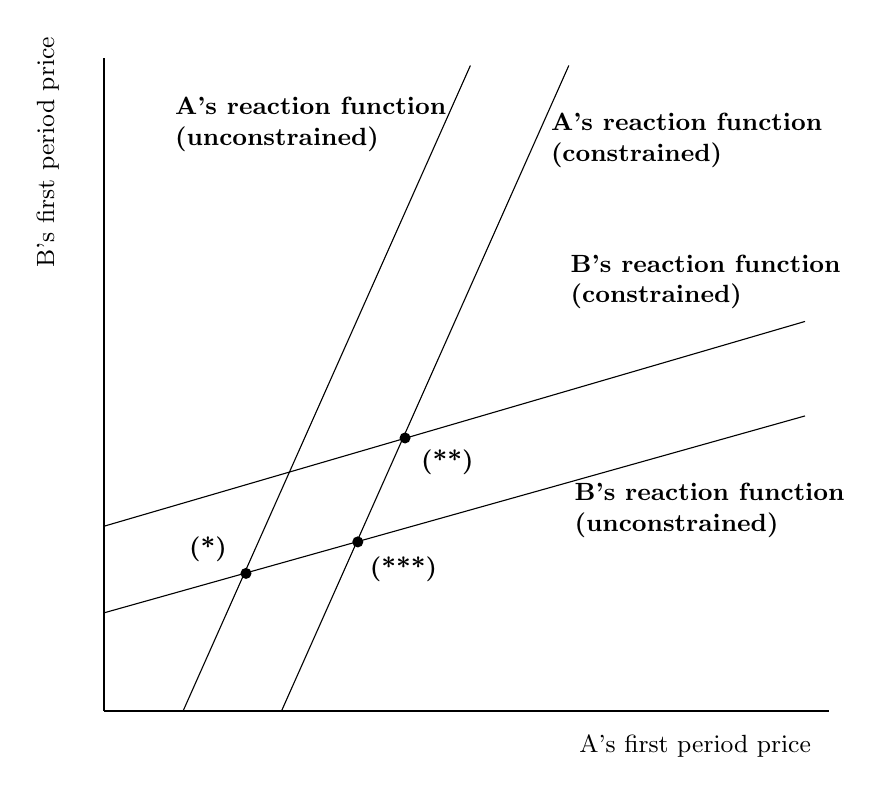
\begin{tikzpicture}[
    x=1cm,
    y=1cm,
    >=stealth,
    every node/.style={font=\small}
]

% Axes
\draw[thick] (0,0) -- (0,8.3);
\draw[thick] (0,0) -- (9.2,0);

% Axis labels
\node[rotate=90, anchor=south] at (-0.45,7.1)
    {B's first period price};

\node[anchor=north east] at (9.1,-0.18)
    {A's first period price};

% ------------------------------------------------
% A's reaction functions: steep lines
% ------------------------------------------------

% A constrained
\draw (1.0,0) -- (4.65,8.2);

% A unconstrained
\draw (2.25,0) -- (5.90,8.2);

% ------------------------------------------------
% B's reaction functions: shallow lines
% ------------------------------------------------

% B constrained
\draw (0,2.35) -- (8.9,4.95);

% B unconstrained
\draw (0,1.25) -- (8.9,3.75);

% ------------------------------------------------
% Labels
% ------------------------------------------------

\node[align=left, anchor=west] at (0.775,7.45)
{
    \textbf{A's reaction function}\\
    \textbf{(unconstrained)}
};

\node[align=left, anchor=west] at (5.55,7.25)
{
    \textbf{A's reaction function}\\
    \textbf{(constrained)}
};

\node[align=left, anchor=west] at (5.80,5.45)
{
    \textbf{B's reaction function}\\
    \textbf{(constrained)}
};

\node[align=left, anchor=west] at (5.85,2.55)
{
    \textbf{B's reaction function}\\
    \textbf{(unconstrained)}
};

% ------------------------------------------------
% Intersection points
% ------------------------------------------------

% (*)
\fill (1.80,1.75) circle (2pt);
\node[anchor=south east] at (1.68,1.78)
    {\textbf{(*)}};

% (**)
\fill (3.82,3.47) circle (2pt);
\node[anchor=north west] at (3.90,3.44)
    {\textbf{(**)}};

% (***)
\fill (3.22,2.15) circle (2pt);
\node[anchor=north west] at (3.25,2.08)
    {\textbf{(***)}};

\end{tikzpicture}
}
    \end{center}
    
    \vspace{0.1cm}

    Denote $e_k$ as an indicator of whether the firm is financailly constrained then:
    \small
    \[\frac{d m^{*A}(e_A,e_B)}{d\mu}=\frac{d p^{*A}(e_A,e_B)}{d\mu}=\left[\left(1-\frac{2e_A+e_B}{3}\right)\theta_H-\theta_L\right]\frac{R-c_2}{\bar{\theta}}.\]
    Markups not neccesarily countercyclical, but finacial constraints increases countercylicality of markups
\end{frame}

\begin{frame}{Oil Shock}
    \label{tab:oil-shock}
    \begin{center}
        \begin{minipage}{\textwidth}
    \centering
    \small
    \renewcommand{\arraystretch}{1.12}
    \begin{tabular}{@{}lccc@{}}
        \toprule
        & \multicolumn{3}{c}{\textbf{Oil Shock Variable}} \\
        \cmidrule(lr){2-4}
        & \shortstack{Oil Exposure\\Dummy}
        & \shortstack{Oil\\Exposure}
        & \shortstack{Change in\\Employment} \\
        \midrule
        National Share $\times$ Oil Shock Exposure
            & $-0.115^{**}$ & $-3.033^{*}$ & $2.267^{**}$ \\
            & $(-2.270)$
            & $(1.724)$
            & $(2.365)$ \\
        \midrule
        $R^2$ & $0.170$ & $0.102$ & $0.130$ \\
        Observations & $100$ & $100$ & $100$ \\
        \bottomrule
    \end{tabular}

    \vspace{0.15cm}
    \centering
    \footnotesize
    \textit{Notes:} The dependent variable is the change in a city's price index from
    1985:Q4 to 1987:Q1.
\end{minipage}

    \end{center}
    \vspace{0.3cm}
    \textbf{Conclusion:} Markups rose more for local chains in oil states.
\end{frame}

\begin{frame}[shrink=8]{1990-1991 Macro-Recession}
    \label{tab:macro-recession}
    \begin{center}
        \begin{minipage}{\textwidth}
    \centering
    \footnotesize
    \renewcommand{\arraystretch}{1.0}
    \begin{tabular}{@{}lc@{}}
        \toprule
        & \textbf{Coefficient} \\
        \midrule
        LBO Share
            & $-0.024$ \\
            & $(0.788)$ \\
        \textcolor{red}{LBO Share $\times$ $\Delta$Employment}
            & \textcolor{red}{$-1.970^{*}$} \\
            & \textcolor{red}{$(1.767)$} \\
        $\Delta$Employment
            & $0.384$ \\
            & $(1.005)$ \\
        $\Delta$Wage
            & $0.0173$ \\
            & $(1.052)$ \\
        Constant
            & $0.010$ \\
            & $(0.864)$ \\
        \midrule
        $R^2$ & $0.095$ \\
        Observations & $59$ \\
        \bottomrule
    \end{tabular}

    \vspace{0.1cm}
    \centering
    \scriptsize
    \textit{Notes:} The dependent variable is the change in a city's price index
    from 1990:Q2 to 1991:Q1.
\end{minipage}

    \end{center}
    \vspace{0.3cm}
    \textbf{Conclusion:} Regions with more LBOs firms raise prices by more in places hard hit by the recession.
\end{frame}

\begin{frame}[shrink=12]{Post Macro-Recession: Firm Level Evidence}
    \label{tab:post-macro-firm-level}
    \begin{center}
        \begin{minipage}{\textwidth}
    \centering
    \scriptsize
    \renewcommand{\arraystretch}{0.92}
    \begin{tabular}{@{}lcc@{}}
        \toprule
        & \multicolumn{2}{c}{\textbf{Coefficient}} \\
        \cmidrule(lr){2-3}
        
            & \textbf{1991:Q1--1991:Q4}
            & \textbf{1991:Q1--1992:Q4} \\
        \midrule
        LBO
            & $0.030^{***}$ & $0.025^{***}$ \\
            & $(3.235)$ & $(2.670)$ \\
        \textcolor{red}{LBO $\times$ $\Delta$Employment}
            & \textcolor{red}{$-1.131^{***}$} & \textcolor{red}{$-0.402^{*}$} \\
            & \textcolor{red}{$(-2.942)$} & \textcolor{red}{$(-1.659)$} \\
        Competitor LBO Share
            & $0.109^{***}$ & $0.120^{***}$ \\
            & $(3.454)$ & $(3.456)$ \\
        \textcolor{red}{Competitor LBO Share $\times$ $\Delta$Employment}
            & \textcolor{red}{$-2.834^{**}$} & \textcolor{red}{$-1.152$} \\
            & \textcolor{red}{$(-2.184)$} & \textcolor{red}{$(-1.389)$} \\
        $\Delta$Employment
            & $0.712^{***}$ & $0.375^{*}$ \\
            & $(2.578)$ & $(1.807)$ \\
        $\Delta$Wage
            & $-0.004$ & $-0.011$ \\
            & $(-0.333)$ & $(-0.892)$ \\
        Constant
            & $-0.003$ & $0.050^{***}$ \\
            & $(-0.413)$ & $(5.044)$ \\
        \midrule
        $R^2$ & $0.179$ & $0.200$ \\
        Observations & $110$ & $89$ \\
        \bottomrule
    \end{tabular}

    \vspace{0.1cm}
    \centering
    \footnotesize
    \textit{Notes:} The dependent variable is the change in a firm's price index
    from 1991:Q1 to 1991:Q4 and from 1991:Q1 to 1992:Q4.
\end{minipage}

    \end{center}
    \vspace{0.1cm}
    \textbf{Conclusion:} LBO firms and firms with LBO rivals raised prices by more in regions hard hit by the recession.
\end{frame}


\begin{frame}{Comments}
    \begin{itemize}
        \item Dynamics limited in model
        \begin{itemize}
            \item Countercyclicality defined as increasing probability of bad state
            \item Why are firms financially constrained?
            \item Procyclicality of financial constraint outside model
            \item However, this simplicity is also part of the elegance
        \end{itemize}
        \vspace{0.2cm}
        \item Methods are simple, but results are robust and idea is ahead of its time
        \begin{itemize}
            \item Recnt empirical work using micro data mostly supports conclusions
            \item In alternative history of the New Keynesian DSGE model, perhaps this paper could have inspired financial amplication to drive markups
        \end{itemize}
    \end{itemize}
\end{frame}
\appendix


\begin{frame}
    \centering
    \vfill
    {\Huge\bfseries Appendix}
    \vfill
\end{frame}

\begin{frame}[allowframebreaks]{References}
    \footnotesize
    \nocite{*}
    \bibliographystyle{apalike}
    \bibliography{cs_1996_references}
\end{frame}

\end{document}
